%!TEX root = ../main.tex
%%%%%%%%%%%%%%%%%%%%%%%%%%%%%%%%%%
% Links:
%
% Difficulty:
% Companies: 
%%%%%%%%%%%%%%%%%%%%%%%%%%%%%%%%%%


%\begin{figure}
%	\centering
%	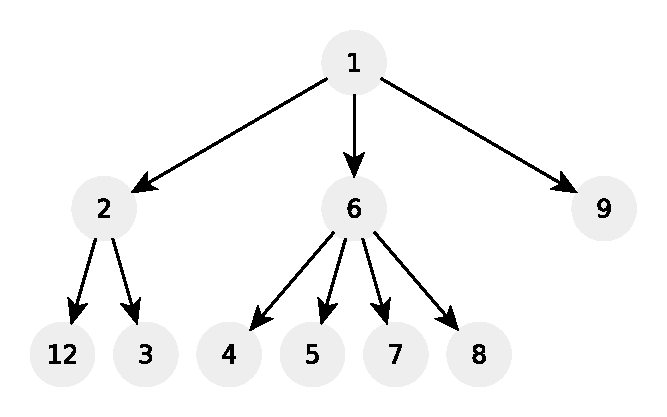
\includegraphics[width=\textwidth]{sources/kth_smallest_in_sorted_matrix/images/example1}
%	\caption[Sample short cpation]{Sample Caption}.
%	\label{fig:kth_smallest_in_sorted_matrix:example1}
%\end{figure}

\chapter{$k^{th}$ smallest element in a sorted matrix}
\label{ch:kth_smallest_in_sorted_matrix}
\section*{Introduction}
\begin{wraptable}{r}{4.5cm}
	\centering
	\begin{framed}  
	\begin{tabular}{|c|c|c|}
	\hline
	1  & 5  & 9  \\ \hline
	10 & 12 & 13 \\ \hline
	12 & 13 & 15 \\ \hline
\end{tabular}%
\caption{Tabular representation of Example \ref{example:kth_smallest_in_sorted_matrix:example1}}
\label{tab:kth_smallest_in_sorted_matrix:example1}
\end{framed}
\end{wraptable} 

One of the most common tool in computer science and engineering in general are rectangular grids of number also known as matrices\footnote{Matrices however are not stored in memory as grids. Computer memory is linear (think of it as a linear array) and therefore matrices must be mapped into it in some way. Turns out there is not only a single way of performing such a mapping, with the most common ones being \textit{row-major} and \textit{column-major}. The row-major stores each rows one after the other contiguously in memory  while column-major does the same but with columns. The matrix in Example \ref{example:kth_smallest_in_sorted_matrix:exercice1} would be stored as $\{\underbrace{1,5,9}_{\text{row 0}},\underbrace{10,12,13}_{\text{row 1}},\underbrace{12,13,15}_{\text{row 2}}\}$ in a row-major mapping and as $\{\underbrace{1,10,12}_{\text{col 0}},\underbrace{5,12,13}_{\text{col 1}},\underbrace{9,13,15}_{\text{col 2}}\}$as column-major.}. The data they  contain can represent many things, from mathematical set of linear equations to algorithm for compression of images and videos or graphs.

In this chapter we are not going to worry about all of those fancy application of matrices and instead we will focus on a much simpler problem on a class of matrices of integers with the property of having rows and columns sorted. The task we need to perform on such a matrix is one that is easily explained: we have to find the the $k^{th}$ smallest number among \textbf{all} values in the matrix.
This is one of such problem for which we will be able to find a working solution straigh-away, but coming up with a more efficient time and space solution is way more complicated. 
On top of that, the naive solution differs conceptually  quite a bit from the faster ones and that further complicates the solution process, especially during an interview. Most of us, once the naive solution is found, are naturally driven towards optimizing it, rather than trying to think about a radically different way to approach the problem which, as we will see is key to yelding solutions with better asymptotic complexity.



\section{Problem statement}
\begin{exercise}
\label{example:kth_smallest_in_sorted_matrix:exercice1}
Write a function that, given an square matrix $M$ of size $n$  where each of individual row and column is sorted in ascending order and an integer $1 \leq k \leq n^2$
returns the $k^{th}$ smallest element in $M$.


You can assume the elements of $M$ to be always in the range $[0,n^2]$.

	%example1
	\begin{example}
		\label{example:kth_smallest_in_sorted_matrix:example1}
		\hfill \\
		Given $M=\{\{1,5,9\},\{10,12,13\},\{12,13,15\}\}$ (as shown in Table \ref{}) and $k=8$ the function returns $13$. See table
	\end{example}
\end{exercise}




\section{Clarification Questions}

\begin{QandA}
	\item Can we assume the input to be always valid i.e. having rows and column sorted?
	\begin{answered}
		\textit{Yes, there is no need to do input validation.}
	\end{answered}
	
	\item Can $M$ contains duplicates?
	\begin{answered}
		\textit{Yes.}
	\end{answered}
	
\end{QandA}

\subsection{Brute-force}
\label{kth_smallest_in_sorted_matrix:sec:bruteforce}
A quick solution to this problem would be to copy into a vector \textbf{all} element of $M$. We can sort this vector and return we will have the answer at location  $k-1$. 
This solution is simple, easy to explain and implement, but most importantly works. Listing \ref{list:kth_smallest_in_sorted_matrix:bruteforce} shows how we can implement this approach.

\lstinputlisting[language=c++, caption={Naive brute-force solution.},label=list:kth_smallest_in_sorted_matrix:bruteforce]{sources/kth_smallest_in_sorted_matrix/kth_smallest_in_sorted_matrix_solution1.cpp}

The code works by copying every single row of $M$ into a temporary array \inline{M_linear} that we then proceed to sort. We can notice how in reality \inline{M_linear} is not really sorted fully, but only partially by using \inline{std::partial_sort}\cite{cit::std::partialsort} (see Section \ref{sec:find_k_closest_in_array:sorting} for another problem where we used this type of sorting) which is called in such a way that the smallest $k$ elements of $M$ are moved to the front of \inline{M_linear} and are properly sorted leaving the rest of \inline{M_linear} unsorted. That is ok because we do not really care about anything but the $k^{th}$ smallest element. We use \inline{std::partial_sort} as this way the overall complexity of this approach is dependent on $k$ instead on the total number of elements in $M$. When $k << |M|$ this can result in measurable performance improvements. However this does not really change the overall time final asymptocical complexity as $K$ can be as big as $M$.
The time and space complexities are therefore $O(nm\times log(nm)$) and $O(nm)$, respectively, where $nm$ is the number of elements in $M$.

\subsection{Brute-force improved}
\label{kth_smallest_in_sorted_matrix:sec:bruteforce_constant_space}
In Section \ref{kth_smallest_in_sorted_matrix:sec:bruteforce} we solved the problem by pure brute-force and we did not take advantage of the fact that rows and columns are sorted to begin with. 
A possible way we can use this fact to our advantage is to use two pointers \inline{rightPtr}, and \inline{downPtr} to navigate rows and columns, respectively. \inline{rightPtr} will always move to the right (thus inspecting rows) and \inline{downPtr} will go downwards to take care of columns. 
Our claim is that we can move these two pointers one at the time, depending on how their pointed values compare to each other and visit $M$ respecting the total order of its elements.
First of all, we should notice that the smallest element will always be at the top-left corner (location $(0,0)$ in $M$).
If we initialize them so that \inline{rightPtr =(0,1)} and \inline{downPtr =(1,0)}, then we know that the \nth{1} smallest element is pointed by \inline{downPtr} and the \nth{2} smallest is the smallest between  \inline{rightPtr} and \inline{downPtr}. Whenever a pointer points to the next smallest element, we move it in its prefeered direction (\inline{rightPtr} to the right and \inline{downPtr} downwards). Of course when a pointer reached the limit of the matrix we make sure to move it either to the next row or column and we make sure to make it start so that we avoid cells that have been already visited. Given \inline{downPtr = (p,q)}, when we need to wrap around \inline{rightPtr= (x,y)} we can move it to \inline{(x+1,q+1)} i.e. to the next row, but avoiding looking at any column that have been already looked by \inline{downPtr}. Similarly, when we need to wrap around \inline{downPtr = (p,q)} we make sure to avoid rows already taken into account by \inline{rightPtr} by setting it to \inline{rightPtr = (x+1,q+1)}. 

If we continue to move these pointers then, after we have moved them $k^{th}$ times we know for sure that one of the two pointers point to the instance's answer and in particular the smallest of the two is the value we need.
Figure \ref{fig:kth_smallest_in_sorted_matrix:visitall} shows how this work using the instance in Example \ref{example:kth_smallest_in_sorted_matrix:example1}.

\begin{figure}
	\centering
	\begin{subfigure}[t]{0.32\textwidth}
		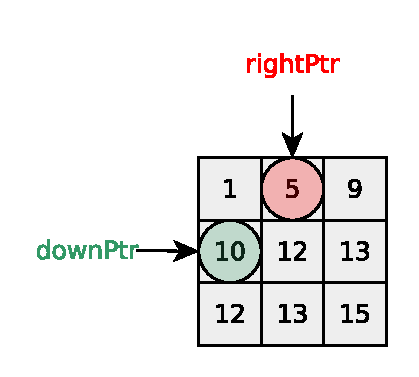
\includegraphics[width=1\linewidth]{sources/kth_smallest_in_sorted_matrix/images/visit1}
		\caption{}
		\label{fig:kth_smallest_in_sorted_matrix:visit1}
	 \end{subfigure}
	\hfill
	\begin{subfigure}[t]{0.32\textwidth}
		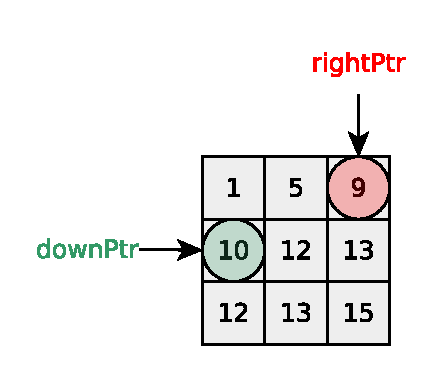
\includegraphics[width=1\linewidth]{sources/kth_smallest_in_sorted_matrix/images/visit2}
		\caption{}
		\label{fig:kth_smallest_in_sorted_matrix:visit2}
	 \end{subfigure}
	 \hfill
	\begin{subfigure}[t]{0.32\textwidth}
		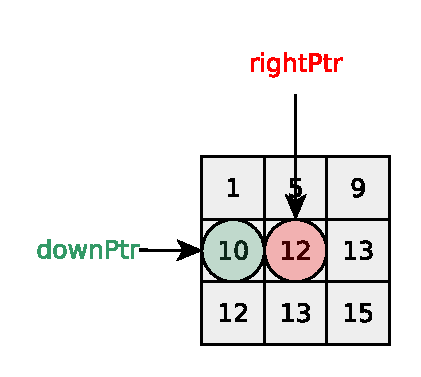
\includegraphics[width=1\linewidth]{sources/kth_smallest_in_sorted_matrix/images/visit3}
		\caption{}
		\label{fig:kth_smallest_in_sorted_matrix:visit3}
	 \end{subfigure}
	 \hfill
	\begin{subfigure}[t]{0.32\textwidth}
		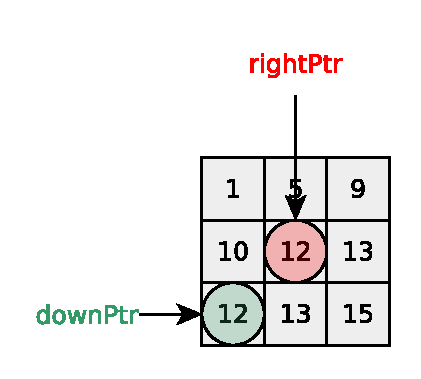
\includegraphics[width=1\linewidth]{sources/kth_smallest_in_sorted_matrix/images/visit4}
		\caption{}
		\label{fig:kth_smallest_in_sorted_matrix:visit4}
	\end{subfigure}
	\hfill
	\begin{subfigure}[t]{0.32\textwidth}
		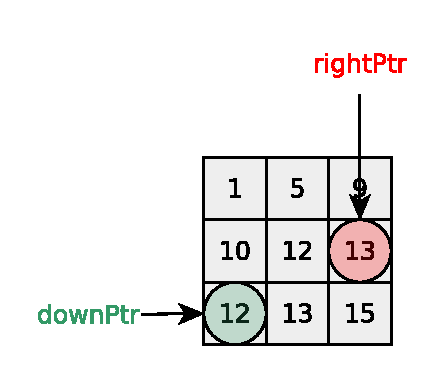
\includegraphics[width=1\linewidth]{sources/kth_smallest_in_sorted_matrix/images/visit5}
		\caption{}
		\label{fig:kth_smallest_in_sorted_matrix:visit5}
	\end{subfigure}
	\hfill
	\begin{subfigure}[t]{0.32\textwidth}
		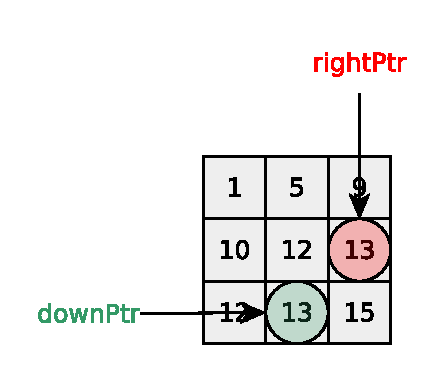
\includegraphics[width=1\linewidth]{sources/kth_smallest_in_sorted_matrix/images/visit6}
		\caption{}
		\label{fig:kth_smallest_in_sorted_matrix:visit6}
	\end{subfigure}
	\hfill
	\begin{subfigure}[t]{0.32\textwidth}
		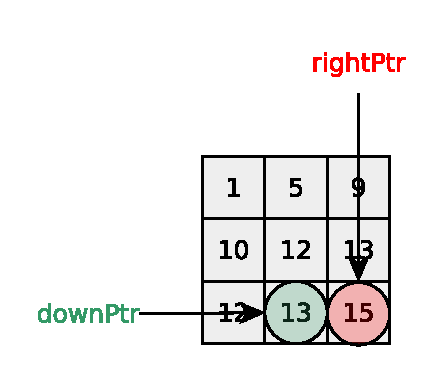
\includegraphics[width=1\linewidth]{sources/kth_smallest_in_sorted_matrix/images/visit7}
		\caption{}
		\label{fig:kth_smallest_in_sorted_matrix:visit7}
	\end{subfigure}
	
	

	 \caption[Execution Listing \ref{list:kth_smallest_in_sorted_matrix} on Example \ref{example:kth_smallest_in_sorted_matrix:example1}]{Execution Listing \ref{list:kth_smallest_in_sorted_matrix} on Example \ref{example:kth_smallest_in_sorted_matrix:example1}. The pointers are initialized as shown in Figure \ref{fig:kth_smallest_in_sorted_matrix:visit1}. We then compare them and move \inline{rightPtr} to the right because it is the smallest among the two of them. Next we move it again as shown in Figure \ref{fig:kth_smallest_in_sorted_matrix:visit2} because the value it points to (i.e. $9$) is still smaller than the value pointed by \inline{downPtr}. We cannot move \inline{rightPtr} to the right as it would break the boundaries of the matrix and we therefore move it one row down but we carefully place it a column to the right of the column \inline{downPtr} is at (because \inline{downPtr} is taking care of that column). After that, in Figure \ref{fig:kth_smallest_in_sorted_matrix:visit4} we can see that  \inline{downPtr} is moved. At this point both pointers point to cells containing the same value. When a case like this happens we always choose to move \inline{rightPtr}. In Figure \ref{fig:kth_smallest_in_sorted_matrix:visit5} we see that \inline{downPtr} is moved again. Notice that, because we could not move it downwards, we moved it one column to the right and to a row below \inline{rightPtr}'s row. Up at this point we moved pointers $7$ times if we also consider cell $(0,0)$ that we skipped entirely. We only need to move it once more to be able to find the \nth{8} smallest. This last step is shown in Figure \ref{fig:kth_smallest_in_sorted_matrix:visit7} where \inline{rightPtr} is moved one row below and one column to the right of \inline{downPtr} column coordinate, finally landing in the last cell.}
	  \label{fig:kth_smallest_in_sorted_matrix:visitall}
\end{figure}

Notice that there could be a case where it is impossible to move a pointer any further as it would go completely outside the boundaries of the matrix on both directions. When this happens, we should simply continue moving the other pointer and keep counting\footnote{We can think of this case as if the exahusted pointer would be always pointing to imaginary cells of infinite value.}.

An implementation of this idea is shown in Listing \ref{list:kth_smallest_in_sorted_matrix:bruteforce_improved}.

\lstinputlisting[language=c++, caption={Brute-force solution using constnat space.},label=list:kth_smallest_in_sorted_matrix:bruteforce_improved]{sources/kth_smallest_in_sorted_matrix/kth_smallest_in_sorted_matrix_solution2.cpp}

The main driver function, \inline{kth_smallest_in_sorted_matrix_brute_force_constant_space} contains a bunch of loos with the first, being the main one. We can see there how \inline{downPtr} and \inline{rightPtr} are compared first and the smallest of the two is moved. In order to move them, two auxiliary functions are used: \inline{advanceDown} and \inline{advanceRight}. These functions make sure the pointers are moved properly, so that if necessary the wrapping around described above is enforced. We can also notice that they return a boolean value which indicates whether the movement resulted in the pointer going outside the boundary of the matrix.
This boolean value is used to break out of the main loop in \inline{kth_smallest_in_sorted_matrix_brute_force_constant_space} and when this happens to decide which pointer needs to be moved further. If \inline{downPtr} went overboard the matrix then we continue moving \inline{rightPtr} and the otherway round if \inline{rightPtr} went overboard.

The time and space complexities of this approach are $O(nm)$ and $O(1)$, respectively, with $nm$ being the total number of cells in $M$.

\subsection{Binary Search}
\label{kth_smallest_in_sorted_matrix:sec:binarysearch}

\lstinputlisting[language=c++, caption={Solution using binary search.},label=list:kth_smallest_in_sorted_matrix]{sources/kth_smallest_in_sorted_matrix/kth_smallest_in_sorted_matrix_solution3.cpp}
